% Gerado automaticamente. No preambulo do documento use:
% \usepackage{pgfplots}
% \pgfplotsset{compat=1.18}
\definecolor{plotblue}{HTML}{2563EB}
\definecolor{plotorange}{HTML}{D97706}
\definecolor{plotgreen}{HTML}{059669}
\definecolor{plotpurple}{HTML}{7C3AED}
\definecolor{plotgray}{HTML}{374151}
\definecolor{plotred}{HTML}{DC2626}
\definecolor{plotteal}{HTML}{0F766E}
\definecolor{plotslate}{HTML}{64748B}

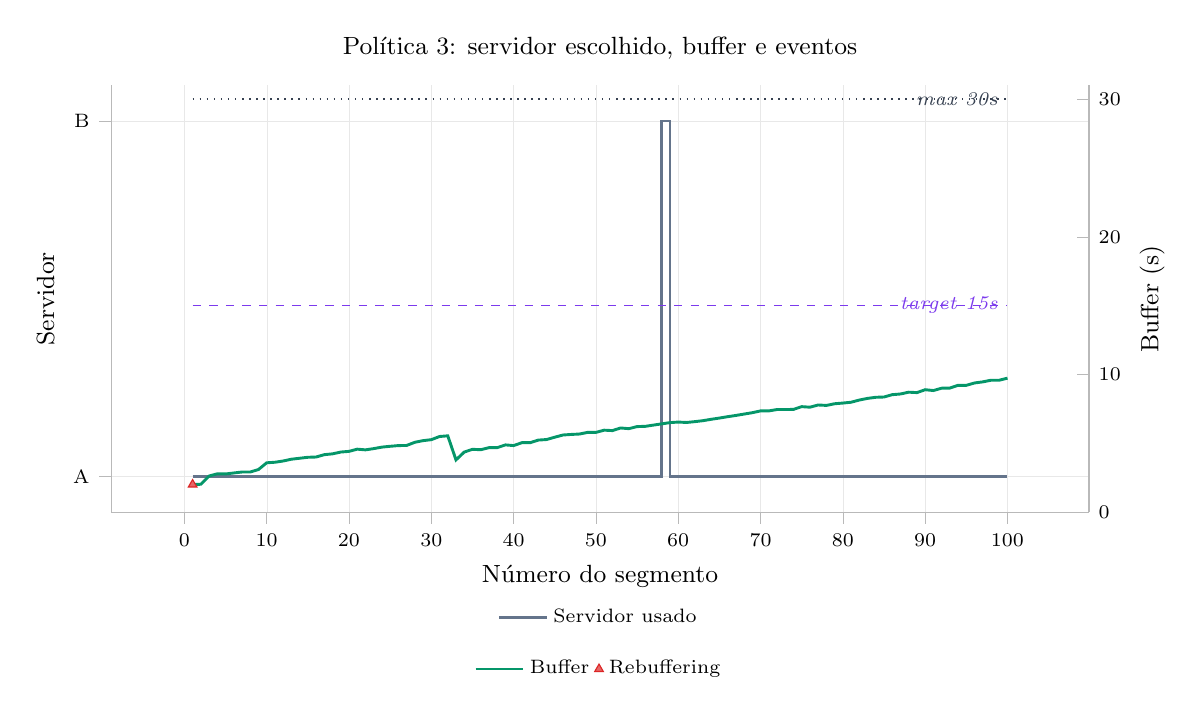
\begin{tikzpicture}
\begin{axis}[
    title={Política 3: servidor escolhido, buffer e eventos},
    xlabel={Número do segmento},
    ylabel={Servidor},
    width=14cm,
    height=7cm,
    grid=major,
    grid style={line width=.12pt, draw=gray!18},
    axis line style={draw=gray!55},
    tick style={draw=gray!55},
    tick align=outside,
    title style={font=\small},
    label style={font=\small},
    tick label style={font=\scriptsize},
    legend cell align={left},
    legend style={at={(0.5,-0.20)}, anchor=north, legend columns=2, draw=none, font=\scriptsize},
    axis y line*=left,
    axis x line*=bottom,
    ytick={0,1},
    yticklabels={{A},{B}},
    ymin=-0.1,
    ymax=1.1
]
\addplot+[plotslate, const plot, line width=1.05pt, mark=none] coordinates {
(1,0)
(2,0)
(3,0)
(4,0)
(5,0)
(6,0)
(7,0)
(8,0)
(9,0)
(10,0)
(11,0)
(12,0)
(13,0)
(14,0)
(15,0)
(16,0)
(17,0)
(18,0)
(19,0)
(20,0)
(21,0)
(22,0)
(23,0)
(24,0)
(25,0)
(26,0)
(27,0)
(28,0)
(29,0)
(30,0)
(31,0)
(32,0)
(33,0)
(34,0)
(35,0)
(36,0)
(37,0)
(38,0)
(39,0)
(40,0)
(41,0)
(42,0)
(43,0)
(44,0)
(45,0)
(46,0)
(47,0)
(48,0)
(49,0)
(50,0)
(51,0)
(52,0)
(53,0)
(54,0)
(55,0)
(56,0)
(57,0)
(58,1)
(59,0)
(60,0)
(61,0)
(62,0)
(63,0)
(64,0)
(65,0)
(66,0)
(67,0)
(68,0)
(69,0)
(70,0)
(71,0)
(72,0)
(73,0)
(74,0)
(75,0)
(76,0)
(77,0)
(78,0)
(79,0)
(80,0)
(81,0)
(82,0)
(83,0)
(84,0)
(85,0)
(86,0)
(87,0)
(88,0)
(89,0)
(90,0)
(91,0)
(92,0)
(93,0)
(94,0)
(95,0)
(96,0)
(97,0)
(98,0)
(99,0)
(100,0)
};
\addlegendentry{Servidor usado}
\end{axis}
\begin{axis}[
    width=14cm,
    height=7cm,
    axis y line*=right,
    axis x line=none,
    ylabel={Buffer (s)},
    ymin=0,
    ymax=31,
    axis line style={draw=gray!55},
    tick style={draw=gray!55},
    label style={font=\small},
    tick label style={font=\scriptsize},
    legend cell align={left},
    legend style={at={(0.5,-0.32)}, anchor=north, legend columns=3, draw=none, font=\scriptsize}
]
\addplot+[plotgreen, line width=1.05pt, mark=none] coordinates {
(1,2)
(2,2.02)
(3,2.62)
(4,2.78)
(5,2.77)
(6,2.84)
(7,2.91)
(8,2.91)
(9,3.09)
(10,3.58)
(11,3.62)
(12,3.71)
(13,3.84)
(14,3.91)
(15,3.98)
(16,4)
(17,4.17)
(18,4.23)
(19,4.36)
(20,4.41)
(21,4.57)
(22,4.52)
(23,4.61)
(24,4.72)
(25,4.78)
(26,4.83)
(27,4.84)
(28,5.07)
(29,5.19)
(30,5.26)
(31,5.49)
(32,5.54)
(33,3.79)
(34,4.36)
(35,4.56)
(36,4.53)
(37,4.68)
(38,4.68)
(39,4.88)
(40,4.83)
(41,5.04)
(42,5.04)
(43,5.23)
(44,5.27)
(45,5.44)
(46,5.6)
(47,5.64)
(48,5.67)
(49,5.79)
(50,5.79)
(51,5.95)
(52,5.92)
(53,6.11)
(54,6.06)
(55,6.21)
(56,6.23)
(57,6.32)
(58,6.41)
(59,6.5)
(60,6.54)
(61,6.51)
(62,6.57)
(63,6.64)
(64,6.74)
(65,6.83)
(66,6.93)
(67,7.02)
(68,7.12)
(69,7.22)
(70,7.35)
(71,7.35)
(72,7.45)
(73,7.45)
(74,7.46)
(75,7.66)
(76,7.62)
(77,7.78)
(78,7.75)
(79,7.87)
(80,7.92)
(81,7.98)
(82,8.14)
(83,8.26)
(84,8.34)
(85,8.36)
(86,8.53)
(87,8.58)
(88,8.71)
(89,8.68)
(90,8.89)
(91,8.83)
(92,9)
(93,9.01)
(94,9.21)
(95,9.21)
(96,9.38)
(97,9.46)
(98,9.58)
(99,9.58)
(100,9.73)
};
\addlegendentry{Buffer}
\addplot+[plotpurple, dashed, line width=0.55pt, mark=none, forget plot] coordinates {(1,15) (100,15)};
\node[anchor=east, plotpurple, font=\scriptsize\itshape] at (axis cs:100,15) {target 15s};
\addplot+[plotgray, dotted, line width=0.55pt, mark=none, forget plot] coordinates {(1,30) (100,30)};
\node[anchor=east, plotgray, font=\scriptsize\itshape] at (axis cs:100,30) {max 30s};
\addplot+[only marks, mark=triangle*, mark size=1.8pt, plotred, mark options={solid, fill=plotred!70, draw=plotred}] coordinates {
(1,2)
};
\addlegendentry{Rebuffering}
\end{axis}
\end{tikzpicture}
